
%(BEGIN_QUESTION)
% Copyright 2010, Tony R. Kuphaldt, released under the Creative Commons Attribution License (v 1.0)
% This means you may do almost anything with this work of mine, so long as you give me proper credit

Anta at en Fisher modell 586 I/P-omformer er satt opp pa benk for en kalibreringstest:

$$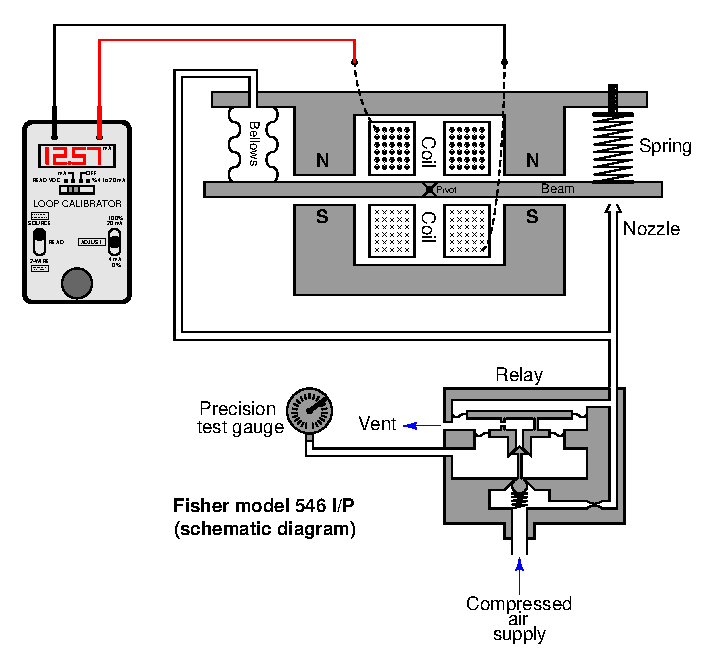
\includegraphics[width=15.5cm]{i00059x01.eps}$$

``Som funnet''-kalibreringstabellen for denne omformeren tester slik:

% No blank lines allowed between lines of an \halign structure!
% I use comments (%) instead, so that TeX doesn't choke.

$$\vbox{\offinterlineskip
\halign{\strut
\vrule \quad\hfil # \ \hfil & 
\vrule \quad\hfil # \ \hfil \vrule \cr
\noalign{\hrule}
%
% First row
Inngangsstrom & Utgangstrykk \cr
%
\noalign{\hrule}
%
% Another row
4.00 mA & 2.97 PSI \cr
%
\noalign{\hrule}
%
% Another row
8.00 mA & 5.98 PSI \cr
%
\noalign{\hrule}
%
% Another row
12.00 mA & 9.00 PSI \cr
%
\noalign{\hrule}
%
% Another row
16.00 mA & 11.37 PSI \cr
%
\noalign{\hrule}
%
% Another row
20.00 mA & 11.37 PSI \cr
%
\noalign{\hrule}
} % End of \halign 
}$$ % End of \vbox

To instrumentteknikere som observerer testen er uenige om arsaken til feilene ved 75\% og 100\%.  Den ene sier at denne omformeren har en {\it spenn}-feil og kan korrigeres ved a justere spennskruen, mens den andre sier at problemet ikke kan korrigeres med noen kalibrering (null eller spenn)-justering.

Hva er din vurdering av instrumentets problem?  Identifiser minst en realistisk arsak, og foresla en utbedring for a rette feilen.

\vfil

\underbar{file i00059}
\eject
%(END_QUESTION)





%(BEGIN_ANSWER)

Dette er et vurdert sporsmal -- ingen svar eller hint gis!

%(END_ANSWER)





%(BEGIN_NOTES)

En god problemlosningsteknikk her er a skissere et diagram av inngangs- og utgangsverdiene for dette instrumentet, for a fa en grafisk representasjon av oppforselen.  Noen ganger gjor dette problemet lettere a se enn a se pa en tabell med tall:

$$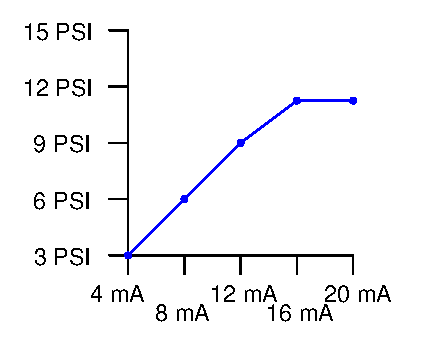
\includegraphics[width=15.5cm]{i00059x02.eps}$$

Fra denne grafen ser vi tydelig at denne I/P-en har en ikke-linearitetsfeil!

\vskip 10pt

Den mest sannsynlige arsaken til problemet er utilstrekkelig forsyningslufttrykk.  Andre mulige arsaker inkluderer feiljustering av kraftbalanse-mekanismen (som far den til a ``kile seg fast'' ved et visst pafoert moment) og en delvis lekkasje i dyseroret et sted (som far dyse-mottrykket til a mette ved et maksimumstrykk lavere enn det burde kunne na).

Den andre teknikeren har rett: dette er i grunn et problem som ikke kan korrigeres med noen skruejustering.  Vi vet dette fordi de tre kalibreringspunktene 4 mA, 8 mA og 12 mA er nesten helt riktige.  Hvis det var et null- eller spennproblem, ville minst to av disse tre punktene {\it ogsa} vare kraftig utenfor spesifikasjon.  Videre vil ingen mengde null- eller spennfeil fa instrumentet til a ``flate ut'' ved 75\% og 100\%-punktene.  En nulljustering ville bare flytte {\it alle} kalibreringspunktene hoyere eller lavere.  En spennjustering vil likeledes pa virke alle kalibreringspunktene til en viss grad, ikke lamme noen mens andre blir nesten perfekte!

Det vi har her er ekstremt ikke-lineaer oppforsel.  Noe hindrer I/P-ens utgangstrykk i a overstige 11.37 PSI.  


%INDEX% Calibration: table, I/P transducer
%INDEX% Relay, I/P transducer: Fisher model 546

%(END_NOTES)



